\documentclass[a4paper,12pt]{article}
\usepackage[margin=2.5cm]{geometry}
\usepackage{setspace}
\onehalfspacing

\usepackage{array}
\usepackage{multirow}
\usepackage{csquotes}
\usepackage[usenames,dvipsnames]{color}
\usepackage[utf8]{inputenc}
\usepackage{pdfpages}
\usepackage{rotating}
\usepackage{longtable}
\usepackage[labelfont=it]{caption}
\usepackage{color}
\usepackage{soul}
\usepackage{amsfonts}
\usepackage{graphicx}
\usepackage{caption}
\usepackage{subcaption}
\usepackage{eurosym}
\usepackage{wrapfig}
\usepackage{titlesec}


\usepackage{titling}
\newcommand{\subtitle}[1]{%
  \posttitle{%
    \par\end{center}
    \begin{center}\large#1\end{center}
    \vskip0.5em}%
}

% Highlight
\definecolor{highlightyellow}{rgb}{1,1,0.7}
\sethlcolor{highlightyellow}
\makeatletter
\newcommand\fix{%
  \let\set@color\beamerorig@set@color
  \let\reset@color\beamerorig@reset@color}
\makeatother

% Note and Source below tables and figures
\usepackage{threeparttable}% Alternative for Notes below table
\newcommand{\Figtext}[1]{%
	\begin{tablenotes}[para,flushleft]
		\hangindent=1em
		\footnotesize
		\raggedright
		#1
	\end{tablenotes}
}
\newcommand{\Fignote}[1]{\Figtext{\emph{Note:~}~#1}}
\newcommand{\Figsource}[1]{\Figtext{\emph{Source:~}~#1}}

% TITLE PAGE
\title{\Large {\bf Auction or haggling -- what should the seller choose?} \\ A look at the interaction between learning and competition in Name-Your-Own-Price auctions.}
\author{Jonas K. Sekamane (LQF640)}
\date{22. December 2014\thanks{This paper is written for the seminar \emph{Experiments in Economics} at the Department of Economics, University of Copenhagen in the autumn 2014. I would like to thank the participants, my supervisor Ulrik Haagen Nielsen (ulrik.haagen.nielsen@gmail.com) and opponent Aksel Thomsen for their questions and comments. Presented the 4. December 2014.}\thanks{See fieldnotes at https://github.com/jsekamane/FixedAuctionNYOP}}

% NEW COMMANDS AND TYPES
\newcolumntype{x}[1]{%
>{\raggedright\hspace{0pt}}p{#1}}%

% Remove heading on TOC
\makeatletter
\renewcommand\tableofcontents{%
    \@starttoc{toc}%
}
\makeatother

% Spacing around headings
\titlespacing{\section}{0pt}{\parskip}{-\parskip}
\titlespacing{\subsection}{0pt}{\parskip}{-\parskip}
\titlespacing{\subsubsection}{0pt}{\parskip}{-\parskip}

% Spacing around equations
\makeatletter
\g@addto@macro\normalsize{%
  \setlength\abovedisplayskip{0pt}
  \setlength\belowdisplayskip{0pt}
  \setlength\abovedisplayshortskip{0pt}
  \setlength\belowdisplayshortskip{0pt}
}
\makeatother

\begin{document}
	
	\pagenumbering{gobble}% Remove page numbers
	\clearpage
	\thispagestyle{empty}
	
	\maketitle{}
		
	\newpage
	
	\begin{abstract}
		{This paper investigates the optimal design choice when selling a single and unique item (such as art, antiques, or collectibles). The paper compares and discusses three price mechanisms: the posted price mechanism, the Name-Your-Own-Price (NYOP) mechanism and the English auction. The first and novel contribution of this paper is the introduction of the NYOP mechanism under supply constraints. The paper proposes a lab experiment that will rank the revenue of the NYOP and the English auction. This comparison of revenue is the second novel contribution of the paper. Additionally the experiment will investigate how the NYOP is affected by competition among buyers and by buyers learning the seller's threshold level. Therefore the experiment focuses on the behaviour of buyers. The third novel contribution of the paper is how competition and learning affect behaviour.}
	\end{abstract}
	
	\tableofcontents
	
	\newpage
	
	\clearpage %  Reset page numbers to 1
	\pagenumbering{arabic}
	\setcounter{page}{1}

	\section{Introduction}

	Which price mechanism should the seller choose? Posted price mechanism, Name-Your-Own-Price (NYOP) or English auction? This article focuses on the selling of unique objects or scarce goods, i.e. where multiple buyers compete for the same object. And so the seller is in essence a monopolist. This area has traditionally been the realm of auctions (art, antiques, collectibles, second-hand, etc). But perhaps the standard single-item auction formats are not the optimal selling methods. An alternative price mechanism is the NYOP. In NYOP the seller sets a posted price and commits to threshold level. Then a buyer proposes a price (bid). If the proposed price is above the threshold level, then the buyer gets the object at his or her proposed price. As shown later, the NYOP can in some cases be thought of as haggling. Haggling and bargaining is usually used to accommodate buyers with low values (Neeman el. at 2013 p.609). %Bargaining can imposes high haggling costs on the seller. The seller can lower his or her exposure to this cost, by allocating the bargaining power to a third party (eg. marketplace or shop assistant). However this in turn opens for principal–agent problems. Advances in information technology has significantly mitigated these problems and costs, such that haggling, and in particular the NYOP, has found its way back into the arena (Terwiesch et. al. 2005 p.339).
	
	All the three price mechanisms are used to sell unique items. The marketplace DBA.dk officially uses a posted price mechanism. But looking through the comments, one quickly realises that haggling takes place frequently. While Lauritz.com sells using a slightly modified English auction. And finally auctionata.com, the largest German online auction house, uses both auctions and NYOP. The NYOP is used for items valued below \euro300.000. %\emph{Why are all three mechanisms prevalent? Why choose one mechanism over the other for low-valued items? If haggling only accommodates buyers with low values, why then use the NYOP to sell single and unique items? Why not officially embrace and improve upon the price mechanism unofficially chosen by sellers and buyers alike?} It is questions like these that have motivated my research into the three mechanisms. The paper will not directly try to answer these questions. It requires other considerations since the marketplaces also differ in inventory, segments, layout, organisational structure and politics, etc. Instead the paper will focus on how the prices mechanisms affect the behaviour of buyers.
	
	A previous experiment by Shapiro and Zillante (2009) shows that NYOP gives the seller a higher revenue than a simple posted price mechanism when there is no constraint on supply. To my knowledge no previous articles on NYOP constrains the supply. Instead there is an item for every buyer, and hence no competition among buyers (see figure~\ref{fig:competition-items}). The lab experiment proposed in this paper tries to answer, if using a NYOP can give the seller a higher revenue than an English auction. But before this, the paper introduces competition into the NYOP, such that it is in fact comparable to the competition found in auctions.  Secondly the experiment tries to understand why -- why revenue is higher in NYOP, or why revenue is not higher? To explain this and the resulting differences between auctions and NYOP, I will compare the main NYOP treatment to three alternative NYOP treatments. In total the experiment will be composed of five treatments (see figure~\ref{fig:treatments}). These are henceforward referred to as $AUCTION_0$, $NYOP_0$, $NYOP_P$, $NYOP_S$, and $NYOP_M$, where the control treatment is $NYOP_0$. All the treatments are explain in detail in section~\ref{sec:treatments}. My hypothesis is that in particular two factors effects the results of the NYOP mechanism: learning and competition. The two factors have counteracting effects on revenue. And by appropriately balancing them, the seller can increase the revenue of the single-unit NYOP. 

{\bf Learning} or price discovery: Through experience and information about previously submitted bids buyers will learn and come to form correct expectations about the seller's threshold level. This will, everything else equal, result in buyers submitting bids closer to the threshold and significantly below the posted price, thus having a negative effect on the seller's expected revenue. I identify three separate channels through which learning happens: 1) the \emph{individual channel} where buyers bid repeatedly and incrementally until they reach the threshold level, 2) the \emph{common channel} where buyers observe what others bid and use this to form expectations about the threshold level, and 3) the \emph{experience channel} where buyers, by participating in multiple rounds, learn the winning bid in each round and from this gradually learn the general distribution of the threshold level.

{\bf Competition}: I introduce competition into the NYOP by reducing the number of items for sale and using an allocation rule henceforward referred to as First-Come-First-Served (FCFS). There are fewer items than buyers creating scarcity and competition. This pressures buyers to submit earlier bids, since only the first bid above the threshold level wins the item. The pressure will, everything else equal, imply that buyers have less time available to discover the threshold level. Hence buyers are not as likely to shade their bids -- or alternatively they disengage from bid-shading, and simply use the `buy' option purchasing the item at the posted price. This will have a positive effect on the seller's expected revenue.

%	This paper is structured as follows. First the prices mechanisms are introduced (posted price, NYOP, haggling, English auction). This section includes a small discussion of how the various price mechanisms relate to one another. Hereafter follows the full description of the experiment: its design, treatments, procedure, participant requirements and expected results. The last sections of this paper includes a recapitulation of my hypotheses, the shortcomings of the experiment, future extensions, and a conclusion.

	\section{Price mechanisms}

	Before diving into the experiment itself, I will set the stage by properly introducing each of the price mechanisms. I will discuss their similarities, introduce notation and concepts. And with this, latter parts of the paper will be more easily understandable.

	\subsection{Posted Price}
	The most common price mechanism is a posted price (also known as {\it listed price} or {\it take-it-or-leave-it offer}). The seller sets the price. The price is visible to all. Buyers can only choose to buy, or choose not to buy. There is often no official count down or time limit on the offer. However the item is usually sold to the first willing buyer (known as \emph{first arrival} or \emph{FCFS}). The posted price mechanism is simple, familiar and generally applicable. In addition to these advantages, the seller has full control over the final price. If sellers are risk averse this may be the decisive feature when settling on a price mechanism. The main disadvantage is the lack of a price discovery process. I.e. what is the optimal posted price for the seller? If the seller sets the price too low, the item is sold quickly and rents may not have been fully exhausted. If its set too high, the item is sold slowly or not at all. Often the seller will be uncertain about the value of the item. Perhaps not the seller's own valuation or reserve price, but uncertain about what the highest value is among all potential buyers. This problem is more prevalent when selling a single and unique item, because there is no prior market price that can guide the seller. In addition buyers may value the exclusivity and the uniqueness of the item, far beyond its mere production costs.

	\subsection{Name-your-own-price (NYOP)}

	\begin{figure}
	        \centering
	        \caption{NYOP game tree}
	        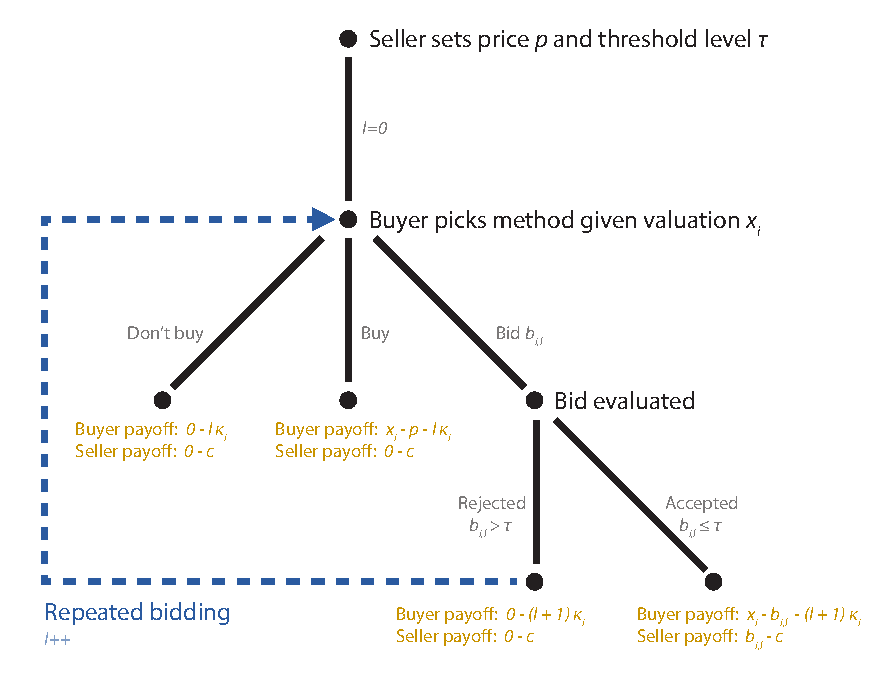
\includegraphics[width=\textwidth]{Figures/NYOP_GameTree}
			\label{fig:game_tree}
			\Fignote{Notation is as follows: $p$ is the posted price, $\tau$ is the threshold level and $c$ is the seller's marginal cost. Buyer $i$ has value $x_i$, and $b_{i,l}$ is the $l$'th bid (e.g. $l$ is the number of bids). And $\kappa_i$ is the haggling cost. Here it is assumed that haggling costs are constant and proportional to the number of bids.}
	\end{figure}

	The name-your-own-price mechanism (also known as {\it reverse pricing} or {\it name-your-own-price auction}) is an extension of the posted price mechanism. The seller decides the posted price and a threshold level at which he or she is willing to sell the item. Only the posted price and the buyer's own value is known to the buyer, who now has one additional option besides `buy', and `don't buy'. The buyers can submit a bid. The bid is rejected if it is below the threshold level. And if above, the bid is accepted and the transaction is made with the buyer. This is the essential parts of the NYOP mechanism, see game tree in figure~\ref{fig:game_tree} (disregard the blue repeated-bidding parts for now). The notation used for NYOP is also presented in figure~\ref{fig:game_tree}. There exist numerous extensions and modifications. %One modification is to hide the posted price, but having less cues about the threshold level just reduces the average bid (Shapiro and Zillante, 2009 pp.731-732). Clearly presenting the posted price has a sort of anchoring effect or acts as a reference price\footnote{In the behavioural economics literature the `anchor' generally does not add any relevant information to the agents decision -- yet the irrelevant `anchor' still affects the outcome of the decision. In NYOP the posted price contains relevant information about the threshold level.}.
	
	The NYOP could be extended by allowing repeated bidding. See the dotted blue-line extension in figure~\ref{fig:game_tree} (there is no immediate payoff when the buyer's bid is rejected). If a bid is reject the buyer can choose to `buy', `don't buy' or `bid' a higher amount. In addition it is normal to assume that buyers endure some non-monetary mental cost or haggling cost from bidding (clicking more buttons, disutility of rejected bid, etc). Terwiesch et. al. (2005) notes that this implies buyers balancing between bidding too much, giving the seller additional rents, and bidding too little, possibly enduring further haggling cost. Or worse wasting haggling cost, if the he or she does not win the item. If the costs are significant, the seller would indirectly be price discriminating buyers based on their haggling cost. I.e. buyers that are more willing to haggle (lower haggling cost) can archive lower prices and higher payoffs. %Terwiesch et. al. (2005 p.342) argue that fairness concerns as well as legal constraints prohibit more systematic price discrimination. The seller cannot price discriminate on other parameters, e.g. the seller cannot change the threshold level based on the identity of the buyer, nor change the threshold based on the bidding sequence. Buyers purchasing an item at the same point in time must be charged the same price.

	The NYOP mechanism has been studied as a method to curb excess capacity or supply. On the internet Priceline.com has been the pioneer of the NYOP mechanism, selling excess hotel capacity and excess seats on planes (Shapiro and Zillante, 2009 p.726). Consequently the literature on NYOP assumes that there are items enough for every buyer willing to make the purchase. There is no constraint on the supply of items and hence no competition among buyers, unlike auctions (Shapiro, 2011 p.4).

	One advantage of the NYOP is that the seller maintains control over the final price, since the lowest possible final price will be the threshold level. Another advantage is that the NYOP has a built-in price discovery process. This process accommodates buyers with values below the posted price, but above the seller's threshold level. They will also be able to purchase. The seller's uncertainty about the value is less critical than under a posted price mechanism, since the seller chooses an optimal price range rather than a optimal price point. If the seller sets the posted price too high, the items may still be sold.

	\subsection{Haggling}

	As previously hinted at, the NYOP mechanism is not far from haggling or models of {\it bargaining}. The NYOP haggling model proposed by Terwiesch et. al. (2005) assumes that the threshold level is constant (as in figure~\ref{fig:game_tree}). %Furthermore they assume that all uncertainties (other buyers' value, other buyers' beliefs, etc) can be lumped together into a single distribution. This way the problem of finding equilibrium simplifies to a problem of search. In this search problem buyers balance between lowering search efforts (by minimising haggling costs or bids) and choosing a bid that is just above the threshold level (by bidding repeatedly and incrementally until a bid is accepted). A key requirement in their model, that allows sellers to charge a price above the marginal cost, is that haggling costs are non-zero.

	More generally in bargaining: 1) agents can enter a mutually beneficial agreement, 2) there is a conflict of interest over the agreement and 3) an agreement cannot be reached without the approval of all agents (Terwiesch et. al., 2005 p.342). Bargaining can been formulated as a procedure where agents sequentially make decisions. Often, even in simple bargaining models, multiple equilibria arise. A distinct difference between what we normally consider as haggling and the repeated-bidding NYOP, is that the seller does not initially set and commit to a threshold level. Instead in haggling the seller evaluates each bid as they tick in. Hence the threshold variable $\tau$ is not necessarily constant (as in figure~\ref{fig:game_tree}), but could be a function of the buyer identity $i$, the number of attempted bids $l$, the sellers impatience, and the set of previously submitted bids by other buyers $b_{j,l}$.

	\subsection{English auction}

	In standard auctions the buyer with the highest bid wins the item. In the English auction bids are open and visible to all. The transaction price is the second highest bid, for this reason the buyer does not shade his or her bid, but in theory bids his or her true value. Buyers continue to incrementally outbid each other until there is no challenger, or until the clock runs out.  There are good theoretical results ranking the revenue of most standard auction formats (Krishna, 2009). And many experimental studies have been carried out trying to confirm these results (Kagel and Levin, 2011). 

	The expected revenue is increasing in the number of buyers. As an example, if the value of buyers is uniformly distributed on $U[0,1]$ and buyers bid their true value, then the expected revenue would the the expected second highest value among buyers, $\mathbb{E}[Y^{(2)}] = (\frac{N-1}{N+1})$. Where $N$ is number of buyers and $Y^{(n)}$ is a stochastic variable of the $n$'th highest value among buyers. In addition, in repeated-bidding such as an English auction, it has been argued that fewer participants leads to less competitive arousal or less `frenzy', and that this in and of itself gives lower prices and lower revenue. This has been referred to as \emph{auction fever} (Ockenfels et. al. 2006 pp.23-24). 

	%Sellers can use a secret reserve price, where buyers only know that a reserve price exists, but not its value. Thus when bidding they need to form expectations about the value of the reserve price. When the auction ends the buyer with the highest bid wins, but only if the bid is above the secret reserve price. I mention the secret reserves price here, since it bears some similarities with the threshold level in the NYOP auction.

	Auctions have many advantages. One is the price discovery process, which may extract additional rents from the buyer, and lead to higher expected revenue that the posted price mechanism. Higher expected revenue specifically happens when the posted price is set below the value of the second highest buyer (Krishna 2009, pp.71-73). With auctions the seller avoids the problem of setting too low a posted price. The price discovery process is an especially appealing feature when selling scarce goods where the seller is uncertain about the value. Another advantage is that standard auctions are efficient since they allocate the item to the buyer with the highest value (see footnote~\ref{footnote:efficient}). A disadvantage is that the seller has no control over the final price. This may especially be problematic for risk averse sellers. Reserve prices or secret reserve price are sometimes proposed as solutions to this, but their effect on revenue remains ambiguous (Haruvy and Leszczyc, 2010. Kagel and Levin, 2011).

	For the experiment I choose the English auction, mainly because this format has most features in common with the repeated-bidding NYOP, hence it is easier to interpret the results as {\it ceteris paribus}. Secondly, because this auction format has an element of learning and competition build in, which is the focus of the additional NYOP treatments. Learning happens in the English auction since bidders can bid repeatedly and see the bids of other buyers, e.g. it has the same three learning channels. Competition is present in all auctions, because of scarce supply and an allocation rule that determines that the buyer with the highest bid wins the item (from now referred to as HIGH). Auctions with `hard close' (a fixed, announced end time) often see sniping behaviour. Buyers simply wait until the very last minutes or seconds before they submit bids. The rationale is that by submitting last-minute bids the buyer does not reveal information to other buyers. Often it will be a small subset of sophisticated buyers that engage in sniping. Since I am not interested in studying the sniping behaviour of a subset of buyers, but rather learning and group learning, the experiment will use randomly varying durations, also known as a {\it candle auction}.

	\section{Experiment}

	Before going into the details of the experiment, I will motivate why the experimental approach is well suited. There are two major problems with the analytical approach. First, the analytical solution often lead to multiple equilibrium or is intractable due to the complexity of the model. Secondly, the actual characteristics of buyers and hence their behaviour is vastly unknown. The literature has well established concepts such as `risk aversion' or `anchoring effect' -- but whether, why or when buyers are risk averse remains a mystery in most settings. %Haruvy and Leszczyc touch upon these issues in their discussion of traditional auctions vs online auctions:
	%\textquote[Haruvy and Leszczyc, 2010 pp.61-62]{\emph{Traditional auction theory builds heavily on bidder rationality, in many cases risk neutrality, bidder symmetry, revenue and strategic equivalences, and other key properties that are … known to be violated in traditional auction settings as well … In our opinion, based on the research reviewed here, questions of optimal design choice in online auctions can often be addressed empirically and have as much to do with bidder preferences, bidder search, mental processing of information, and issues of trust and reputation as they do with the traditional focus on equilibrium predictions.}}

Although the posted price mechanism has enter the discussion on equal footing with NYOP and English auctions so far, in the experiment only the latter two mechanisms will be investigated. Primarily to maintain a feasible number of treatments, but secondly the posted price mechanism with a FCFS, is unlikely to return interesting results. 

Although the paper has discussed haggling costs, and theoretical results hinge on them, haggling cost are not imposed in the experiment\footnote{There are several reasons for this. First, the haggling costs are assumed to be non-monetary (clicking more buttons, disutility of rejected bid, etc.). It might be possible to convert these non-monetary cost into some monetary amount, but there is no agreement on the conversion ratio, functional form of haggling costs (linear or nonlinear in the number of bids), and no guarantee that haggling costs are identical across buyers. Any conversion or monetary amount would be completely arbitrary. Second, when haggling costs are not imposed one can at least afterwards see whether haggling costs are zero or non-zero (similar to Shapiro and Zillante, 2009).}.% Third, since supply is constrained in the NYOP mechanism, non-zero haggling costs should not be necessary for the seller to archive a price above marginal costs. Fourth, it would hamper comparisons with the English auction, or alternatively one would have to impose haggling cost in the English auction as well. Which in turn would hamper comparisons with other experimental and theoretical results.}. 

	\subsection{Design}
	\label{sec:design}

	This experiment is interested in studying the behaviour of buyers under different mechanisms. Participants in the experiment all play the role of buyers. To simplify and control for the behaviour of the seller, the actions of the seller is carried out by a computer. The seller chooses a posted price and threshold level.

	\begin{wrapfigure}[9]{r}{0.6\textwidth}
	%\begin{figure}[h]
	        \centering
	        \caption{Overview of values and distributions}
	        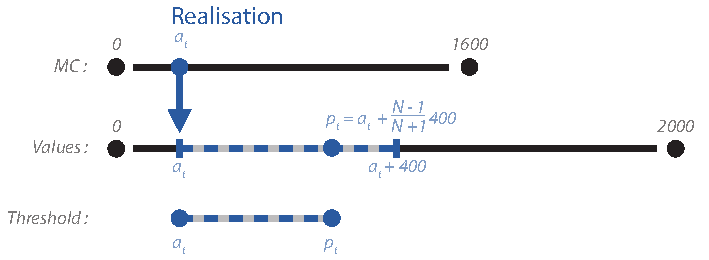
\includegraphics[width=0.6\textwidth]{Figures/Distribution}
			\label{fig:distribution}
	%\end{figure}
	\end{wrapfigure}

	In each round $t$, the values of buyers, the seller's posted price and threshold level are randomly drawn from uniform distributions, see figure~\ref{fig:distribution}. In each round the buyers' values are drawn from $U(a_t , a_t + 400)$, where $a_t$ is drawn from $U(0, 1600)$. The lowest value distribution in any round thereby becomes $U(0, 400)$ and the highest $U(1600, 2000)$ and overall values can range between 0 and 2000. This price range resembles the low-valued and majority of items found on dba.dk, lauritz.com and auctionata.com. Buyers only see their own value and the posted price, they do not receive any information on the distributions. The posted price is set equal to the theoretical expected second highest value of buyers, $p_t = a_t + \frac{N-1}{N+1}400$. On average the English auction should thus give the posted price. As discussed below the NYOP mechanism will on average also give the posted price, if the effect of competition is sufficiently strong. The seller's marginal cost is $a_t$. The threshold level is drawn from $U(a_t, p_t)$. By randomising variables it will be possible to normalise and test which affect the various values of buyers have on the results. In the English auction only the buyers' values and posted price is used. There is no reserve price or secret reserve price, but bids have to be strictly positive.
	
	\subsection{Posted price and number of bidders}

	\begin{figure}
	        \centering
	        \caption{Simulation of final price in auction and NYOP for varying number of buyers}
	        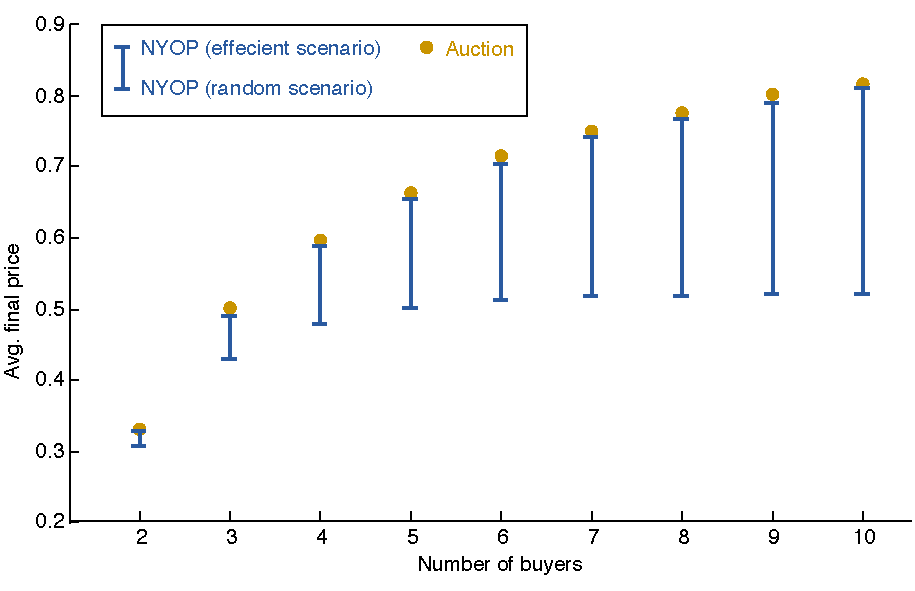
\includegraphics[width=0.7\textwidth]{Figures/FinalPrice_Auction-NYOP}
			\label{fig:FinalPrice_Auction-NYOP}
			\Fignote{In the NYOP the posted price is the theoretical expected second highest value of buyers: $\frac{N-1}{N+1}$.}
	\end{figure}
	
	 To my knowledge there exists no theoretical or empirical evidence guiding the seller on how to set the optimal posted price in the NYOP mechanism\footnote{The literature instead focuses on the optimal threshold level. From theoretical models Fay (2004) and Terwiesch el. at. (2005) respectively derive the optimal threshold level in the repeated-bidding NYOP. Shapiro and Zillante (2009) set the posted price equal to the monopoly price (mid-point of buyers' value range), but note that it might be sub-optimal. In all three articles they only consider the NYOP under excess supply.}. Under supply constraints it seems logical that the seller sets an optimal posted price such that it is increasing in the number of expected buyers, since more buyers increase the likelihood of encountering a buyer with a high value. Given that there are no guidelines to follow, when selecting the optimal posted price, I have chosen to set the posted price equal to the expected price in the English auction. In the English auction the theoretical expected price is the expected second highest value among buyers, $\mathbb{E}[Y^{(2)}] = \frac{N-1}{N+1}$ when values are distributed $U[0,1]$ and buyers bid their true value.

	Figure~\ref{fig:FinalPrice_Auction-NYOP} presents the results of a Monte Carlo simulation, where the number of buyers range from 2 to 10. The simulation uses the distributions described in section~\ref{sec:design} and figure~\ref{fig:distribution}, but the value of buyers is drawn from $U[0,1]$ for simplicity. I have simulated 10.000 rounds and calculated the average of the second highest value of all rounds (the dots labelled `Auction'). Similarly I have calculated the average for the NYOP. In the NYOP I have assumed that buyers are rational and thus use the `buy' option if their value is above the posted price. Buyers with values below the threshold level are not able to purchase an item, and thus not included in the average. The FCFS allocation rule makes it difficult to predict which buyer will ultimately purchase the item. Therefore I have calculated two scenarios, that reasonable well resembles an upper and lower bounds on the average price. The `efficient scenario' assumes that the buyer with the highest value in each round manages to purchase the item -- this provides an upper bound. The `random scenario' assumes that in each round, each buyer is equally like to purchase the item. And it uses the average value of buyers in each round -- this resembles a lower bound. The actual price in the experiment will depend on the respective forces of competition and learning. If the effect of learning is sufficiently strong, then the price should be closer to the expected threshold level $\mathbb{E}[\tau_t]] = \frac{N-1}{(N+1)2}$. If competition is sufficient strong, such that buyers overwhelmingly use the `buy' option instead of engaging in bid-shading, then the price should be closer to the upper limit. And thus reasonably close to the price of the English auction. In sum with this posted price, comparisons between NYOP and the English becomes straight forward, and provides easily testable hypotheses:

	\noindent\fbox{\parbox[b][4em][t]{\textwidth}{\emph{Hypothesis 1:} If the effects from competition is sufficiently strong to outweigh the effects from learning, then the expected revenue from the repeated-bidding single-unit NYOP is the posted price. That is $\mathbb{E}[R^{NYOP_0}] \approx P$.}}

	If the hypothesis fails, I expect lower revenue, but not on average below $\mathbb{E}[\tau_t]]$.

	\noindent\fbox{\parbox[b][5.5em][t]{\textwidth}{\emph{Hypothesis 2:} If competition is sufficiently strong (hypothesis 1). Then by carefully selecting the posted price, the seller can achieve the same revenue in the repeated-bidding single-unit NYOP as in an English auction. That is $\mathbb{E}[R^{NYOP_0}] \approx \mathbb{E}[R^{AUCTION_0}]$ when the posted price is set as $P = \mathbb{E}[Y^{(2)}]$.}}
	
	If the hypothesis above fails I expect the English auction to give a higher revenue than the repeated bidding NYOP. On the other hand, if the hypothesis is true it implies that there might be a range of optimal posted prices above the expected second highest value $P \in (\mathbb{E}[Y^{(2)}], \bar{P})$, for which the NYOP mechanism outperforms the English auction. And that this could be within reach if the seller has a fairly good estimate of the number of buyers and the distribution of their values. The experiment would provide no information on the upper limit on this optimal posted price range $\bar{P}$, but would leave this open for future research.
	
	Each session will have 5 participants ($N=5$). This seems to strike a good balance, such that there is sufficient competition without creating too much frenzy. I feel confidant that I have managed to sufficiently controlled for the number of buyers, such that my results are not a product of the exact number. But this requires formal testing, e.g. by re-running the experiment with different number of buyers. Similarly when determining the external validity of the experiment, one should be cautious due to the complication of the arrival process of buyers, as discussed in section~\ref{app:perspective}.

	\subsection{Treatments}
	\label{sec:treatments}

	There are five treatments see figure~\ref{fig:treatments}, referred to as $AUCTION_0$, $NYOP_0$, $NYOP_P$, $NYOP_S$, and $NYOP_M$. The $NYOP_0$ treatment is the control. The two main treatments are: English auction ($AUCTION_0$) and NYOP ($NYOP_0$).
	In both buyers can repeatedly submit bids (repeated bidding). The auctions ends when the clock runs out, and the winner is the highest bidder. In the NYOP a buyer can `buy' or submit a bid, if the bid is above the threshold level, the buyer wins the object and the auction ends. If the bid is rejected, the buyer can `buy' or resubmit a new higher bid. This is the \emph{individual channel} in which learning can happen. The NYOP ends once a buyer uses the `buy' option or once the seller receives a bid above the sellers threshold level. If no one buys or if no successful bid is submitted then the NYOP ends when the clock runs out. In both treatments all previously submitted bids are visible to all (affiliated values). Buyers can use this information to form and update expectations about the value of other buyers and about the seller's threshold level (in NYOP). This is the \emph{common channel} through which learning can happen. Once the object is sold and the round ends, the posted price along with the winning bid is displayed to all buyers, before the next round initiates. Displaying this information hopefully helps minimise the effects of expectation errors. And strengthens learning through the \emph{experience channel}. In both treatments a single unique unit is put up for sale (single unit). This together with the respective allocation rule introduces competition into both treatments. The three additional NYOP treatments, trying to disentangle the counteracting effects of learning and competition.

	{\bf Multiple unit treatment} ($NYOP_M$). 
	
	\begin{wrapfigure}[7]{r}{0.7\textwidth}
	%\begin{figure}[h]
	        \centering
	        \caption{Competition and number of items for sale}
	        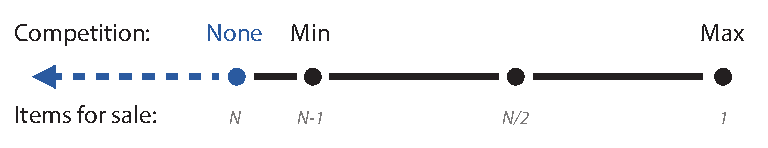
\includegraphics[width=0.7\textwidth]{Figures/Competition-Items}
			\label{fig:competition-items}
	%\end{figure}
	\end{wrapfigure}
	
	By selling multiple units rather than a single unit competition among buyers is reduced, while the learning is unaffected. Winning bids are only displayed after the round ends, while bids below the threshold level are still shown to all. Buyers are not told how many unsold items remain, only the total number of units for sale. When the round ends the posted price and all winning bids are shown. Purchase prices and number of sold items are hidden until after the round ends, such that buyers have the same information as in $NYOP_0$. Minimum competition is as attended by selling $N-1$ units, and maximum by selling 1 unit. The multiple object treatment will sell $ceil(N/2)=3$ units, see figure~\ref{fig:competition-items}. Competition changes in the multiple item treatment, while learning is unaffected. Compared to $NYOP_0$ changes in revenue will be due to decreased competition among buyers.

	{\bf Single bid treatment} ($NYOP_S$).
	In this treatment buyers are only allowed to submit one bid. If the bid is rejected they cannot resubmit a new nor buy. This restriction removes the buyer's ability to learn the threshold level through the \emph{individual channel}. It is still possible to learn through the \emph{common channel}. That is, buyers can still discover the threshold level, but it requires waiting for other buyers to submit their bids, and while waiting they risk that others win the object. It is still possible to learn through the \emph{experience channel}. The number of buyers might be crucially here, since faced with more competing buyers, buyers will be more hesitant to wait. Competition among buyers is not affected in the single bid treatment. Changes in revenue will be due to decreased price discovery, e.g. no learning taking place through the \emph{individual channel}.

	{\bf Private value treatment} ($NYOP_P$).
	Another way in which price discovery can change is by restricting the \emph{common channel}. This is the purpose of the private value treatment. Here buyers can only see their own bids. Buyers still have the ability to learn the threshold level though the \emph{individual channel}, but they now have less information about competing buyers. Comparing the results from this treatment with the previous treatment and $NYOP_0$ will answer how buyers discover the threshold level -- if it is by individually and repeatedly submitting bids or mainly through observing what others bid. 
	
	\subsection{Procedure of experiment}
	
	Each session has 5 treatments, and 8 rounds per treatment. Each participant goes through a total of 40 rounds. 8 rounds should be sufficient to uncover if learning takes place through the \emph{experience channel}, and not too long, such that it demotivates participants. The duration of each round in seconds is drawn randomly from the uniform distribution $U(60, 120)$. Participants will be told that the duration varies, and told that ``each rounds may last a couple of minutes'', but otherwise not be given any information about the distribution. There is no visible countdown. This is done to avoid sniping and encourage early bidding in the English auction. The NYOP treatments may end before the clock runs out, if all items have been sold. The order of treatments will vary with session. By varying the order one can afterwards test and ensure that the results are not due to one particular ordering (known as spillover effects). Four of the orders have been selected at random, but with the requirement that the auction treatment is either first or last. Since different instructions are needed, and to give participants a coherent experience. Sessions will use one of the five orderings found in table~\ref{tab:order}.
	
	The experimental procedure is structured as follows: at the beginning of the session participants are given instructions to either the first auction treatment or the first 4 NYOP treatments. Once these are over, the participants are given instructions to the remaining treatment(s). Each new treatment is announced before it begins so participants are aware of the change in environment. %At the end of the session two treatments are randomly drawn and participants are paid based on their total earnings in those two treatments (see section~\ref{sec:participants-payment}).

	\subsection{Participants and payment}
	\label{sec:participants-payment}
	The participants will be students. The experiment will be carried out in the computer lab at the University of Copenhagen. The computer lab has a capacity of 40 students. The experiment will be run over 5 days, such that a total of 200 students will complete a total of 40 sessions (8 sessions for each treatment order). The experiment will be build in ztree. Prior knowledge about auctions is not a requirement, nor an impediment to participation. Countless studies have successfully conducted experiments on auctions and competition using students. The only restriction on participants, is with regards to the learning effects. That is how participants come to form expectations about a threshold level that is drawn from an uniform distribution. This requires that participants have no prior knowledge of the distribution. So a participant can take part in no more than one session.
	
	Participants are given a show-up fee of 50 kr. In addition participants are paid based on their performance. The performance payment is based on two randomly selected treatments of the five treatments. By randomising -- such that participants have no \emph{a priori} knowledge of which exact treatments their payments will be based on -- I hope to keep participants on their toes and engaged throughout the entire session. In addition the payment schedule is selected so it is easy for participants to convert values and prices observed in the experiment into danish kroner. Hopefully this will strengthen the relation between actions in the experiment and the final monetary payment. The performance payment is calculated as the one-tenth of the differences between the buyer's values and the transaction prices (posted prices or bids) for the items that the buyer successfully purchases. The payment is zero in the rounds were the buyer does not manage to purchase an item. This could happen if the buyer's value is below the threshold level, if the buyer is slower than other buyers, or if another buyer outbids in the auction. Table~\ref{tab:payment} provides examples illustrating how a buyer's payment would look in four different rounds.
	
	The expected payments are 17 kr. and 41 kr. for a round in respectively treatment $AUCTION_0$ and $NYOP_M$. The expected payments is 14 kr for a round the treatments $NYOP_0$, $NYOP_S$, $NYOP_P$. See calculations in the appendix~\ref{app:expected_payment}. In each session with 8 rounds per treatment, and taking account of the combinatorics, a participant can therefore expect a total payment of $50 + \frac{(17+14)3 + (17+41) + (14+14)3 + (14+41)3}{10}8 = 50 + 320 = 370$ kr. While the expected performance payment is quite high so is its variance, since 4 participants are paid zero in every round (in four of the treatments).
	
	\subsection{Evaluating results of experiment}
	
	I first normalise using the realised marginal costs $a_t$ from each round. By subtracting the realised marginal cost from the value of buyers, values will be distributed on similar interval $U[0,400]$ in all rounds and treatments. Similarly by subtracting, the normalised posted price will be $p = \frac{N-1}{N+1}400$. Bids and threshold levels are also normalised. 

	Revenue comparisons between the different treatments is done using a Student's t-test, more specifically the Welch's t-test. I compare mean revenue\footnote{\label{footnote:efficient}One could also evaluate and compare the efficiency of $NYOP_0$ and $AUCTION_0$ treatments. However this seems unproductive, as the NYOP would most likely be inefficient. In an efficient allocation the buyer with the highest values gets the object. However the FCFS allocation rule does not promote efficiency.}. Note that the item might not be sold in every NYOP round. This event is rare, but could happen for particular realisations where the value of all buyers is below the threshold level. $\mbox{Prob}[Y^{(1)} \le \mathbb{E}[\tau]] = \left(\frac{N-1}{(N+1)2}\right)^N$ or approximately 4\% of all cases with five buyers. Descriptive statistics on the percentage of unsold items will be calculate to evaluate if unsold items could have influenced the results. For the multiple item NYOP treatment ($NYOP_M$) the average revenue of the 3 items sold is used. Shapiro and Zillante (2009) find that an important factor increasing revenue in the NYOP is the participation of `new buyer' with values below the posted price. The fraction of `new buyers' that manage to acquire the item will surely affect the results of the NYOP treatments. Descriptive statistics for this will also be calculated.

	I analyses the behaviour of bidders using 1) descriptive statistics on the average bid size, 2) a regression on bid size, and 3) a regression on the probability that buyers `buy' without submitting a bid. By comparing the results across treatments I can determine the effect of learning. In particular in the $NYOP_0$ treatment learning happens through all three channels, while $NYOP_S$ only contains the \emph{common} and \emph{experience channel}, and $NYOP_P$ only contains the \emph{individual} and \emph{experience channel}. Thus resulting differences between these three treatments will be due to learning through respectively \emph{individual} and \emph{common channel}. The effect of the \emph{experience channel} is estimated by looking at bidding across rounds $t$. To determine which factors influence the individual bidding behaviour a fixed effect panel-data estimation is run separately for each treatment. The dependent variable is the bids of buyer $i$ and the buyers identity is the fixed effect:

	\[ b_{t,i,l} = \beta_0 + \beta_1 i + \vec{\beta_t} \vec{t} + \vec{\beta_l} \vec{l} + \beta_2 x_{t,i} + \beta_3 p_t + \beta_4 won_{t-1,i} + \beta_5 bought{t-1,i} \]

	Bidding is explained by the buyer's value $x_{t_i}$, the posted price $p_t$, a dummy equal one if the buyer won the item last round trough bidding $won_{t-1,i}$, and a dummy equal one if the buyer bought the item last round $bought{t-1,i}$. The third and fourth term is the round $t$ and the number of bids $l$. There are 8 rounds in every treatment, if learning takes place through the \emph{experience channel} one should expect that bids decrease as the buyer participated in more rounds and gained more experience. The vector $\vec{\beta_t}$ should contain decreasing values. The values in vector $\vec{\beta_l}$ should be increasing, since buyers bid a higher amount, if a previous bid is rejected. This is not that interesting, but expanding the model by including interactions terms between the number of bid $l$ and other variables, or including the number of bids $l$ in a non-linear fashion, could be fruitful. To determine buying behaviour a fixed effect panel-data logit estimation is run separately for each treatment. The dependent variable is a dummy that takes one if the buyer bought the item without submitting any bids:

	\[ \mbox{Prob}[bought_{t,i} | b_{t,i} = \emptyset]  = \beta_0 + \beta_1 i + \vec{\beta_t} \vec{t} + \beta_2 x_{t,i} + \beta_3 p_t \]

	
	\section{Conclusion}
	This paper introduces of the NYOP mechanism under supply constraints. Proposes an experiment that compares the revenue of the NYOP and English auction. In addition the experiment investigates how the NYOP is affected by competition among buyers and by buyers learning the seller's threshold level.
		
	%shortcomings of the experiment
	%- Sellers behaviour: The optimal threshold level of sellers. Can sellers threshold level actually be thought of as drawn from some distribution, where there is a clear connection to value of buyers and the posted price. If sellers, do not commit to a threshold level, but are able to evaluate the bids of buyers, how will this then affect the results.
	
			
	\newpage
	\appendix
	
	\begingroup
		\section{References}
		\bibliographystyle{apalike-url}
		\nocite{*}
		\renewcommand{\section}[2]{}%
		\raggedright
		\bibliography{ref}
	\endgroup
	
	\newpage
	\section{Appendix}
	
	\subsection{Putting NYOP into perspective}
	\label{app:perspective}

	This section contains a review of the theoretical and experimental results in the literature. The review is very selective due to space limitation. Note that supply is unconstrained in all the articles on NYOP, and it is not clear how or if their results carry over to a NYOP mechanism with competition.
	% With emphasis on explaining difference in revenue between the posted price, NYOP, and auctions. Some attention will also be given to learning in the NYOP. 

	{\bf NYOP vs posted price mechanism}. The experiment by Shapiro and Zillante (2009) find that revenue is higher in NYOP than under the posted price mechanism. The price presented in the NYOP should act as an upper limit on the final price, and one might intuitively have expected that revenue was lower. E.g. buyers that could afford the posted price, would use the NYOP option in an attempt to get the item cheaper. It is in fact a weakly dominant strategy to bid in the setup of Shapiro and Zillante (2009), since buyers can `buy' after their bid has been rejected. What drives their results is 1) new buyers, that could not afford the item at the posted price (e.g. higher quantity of sold items), and 2) buyers with values much higher than the posted price that still use the `buy' option and pay the posted price. They explain the latter with non-monetary mental cost or haggling cost associated with bidding which buyers avoid when they use the `buy' option.

	Similarly {\bf buyout auctions} or a {\it buy-it-now} price in auctions adds an upper limit on the final price. The buyout option has been popularised by internet marketplaces such as eBay. Besides bidding in the auction as described earlier, buyers have the option to purchase the item at the posted price ending the auction before the clock runs out\footnote{Temporary {\it buy-it-now} option can also be found on eBay, here the {\it buy-it-now} option disappears once the auction receives its first bid.}. It has puzzled researchers, that the seller would choose to cap their expected revenue by using a {\it buy-it-now} price. One possible explanation is that when buyers are risk averse, a carefully selected price under {\it buy-it-now} may increase revenue. It does so by extracting the risk premium that buyers are willing to pay to avoid losing the auction (Kagel and Levin, 2011). Another possible explanations is that sellers use the {\it buy-it-now} to extract buyers participation costs, in that buyers choose the buy-it-now option if their time-sensitivity or transaction costs is sufficiently large. Or using, a carefully selected {\it buy-it-now} price as a reference price to influence and increase the value of buyers. For further explanations see Haruvy and Leszczyc, 2010 pp.17-23 and Kagel and Levin, 2011 pp.88-89. The explanations above may also provide answers to why buyers choose `buy' over `bid' option in the NYOP. And why, with a carefully selected posted price, the NYOP may generate higher revenue than an auction.

	The {\bf duration} of the auction is an important parameter, especially in internet auctions that can stretch over several days. In long-duration auctions the individual buyer takes his or her time-sensitivity or impatience into account when bidding. Secondly, the duration of the auction may affect the discovery process of the auction. If one imagines that the process by which buyers discover an auction is random, then the longer the duration, the more buyers will find and participate in the auction, which should lead to higher revenue. Haruvy and Leszczyc (2010) summaries a field experiment conducted on eBay and at a local auction platform. The experiment finds that on eBay a longer duration results in higher revenue, while the opposite is true at the local auction. Haruvy and Leszczyc (2010) argue that this is due to the random arrival process at eBay auctions, while the local auction attracts buyers in higher concentrations by sending out invitations. Therefore a longer duration at the local auction does not lead to more participants -- but just less competitive arousal and less \emph{auction fever}, thus lower revenue.

	Haruvy and Leszczyc (2010) do not make the connection, but this finding may actually describe when and why a posted price mechanism is preferable to an auction. Or for that matter when the NYOP mechanism is preferable to an auction. In auctions the revenue depends critically on the competitive and synchronous interaction of buyers, while this is less true for mechanisms that use a FCFS allocation rule. If the arrival time of buyers is long, then the seller should also have a long time frame on the auction, such that more buyers participate, increasing the revenue. But if \emph{auction fever} is a significant force driving up prices, then too long a time frame may have negative effects on revenue. Because of less competitive arousal of buyers, leading to lower bids or less out-bidding. The seller should balance these two counteracting effects when deciding on the optimal duration of an auction. It seems reasonable to assume that in many cases the seller can not significantly influence the arrival process of buyers. In conclusion there might be arrival process (like long arrival times) of buyers were auctions are not the optimal mechanism. This could explain why auctionata.com uses the NYOP for low-valued items where the arrival time of buyers presumably is longer. And use auctions for high-valued item where the natural arrival time is short, or where auctionata.com may be able to influence the arrival time of buyers (through invitations, events, advertisement, newsletters, etc). Under FCFS, competition among buyers is primarily driven by the fear that another buyer will manage to purchases the item first. This also depend on the arrival process of buyers, but perhaps less so than \emph{auction fever}. It would be interesting to further investigate this train of thought, but it is beyond the scope of this paper and its experiment.

	%Shapiro and Zillante (2009, p.737) hypothesis that the fear of buyers learning the threshold level might be the reason why some NYOP marketplaces have an opaque feature (exact characteristics of the product are not presented to buyers) while others do not. The customers of Priceline are likely to travel from NYC to Los Angeles many times, and hence learn the threshold level through the \emph{experience channel}. Hence Priceline uses the opaque feature, while prisminister.dk that sells consumer electronics does not -- it is less likely to buy washers repeatedly.

	%Haruvy and Leszczyc (2010) argue that finding the optimal posted price requires product-category expertise and knowledge of the competitive situation. And that the posted price mechanism should be preferable to an auction for highly specialised or experienced sellers.

	\newpage
	\subsection{Stylised illustration of treatments}
	\label{app:stylised_treatments}
	
	\begin{figure}[h]
	        \centering
	        \caption{Overview of the five treatments}
	        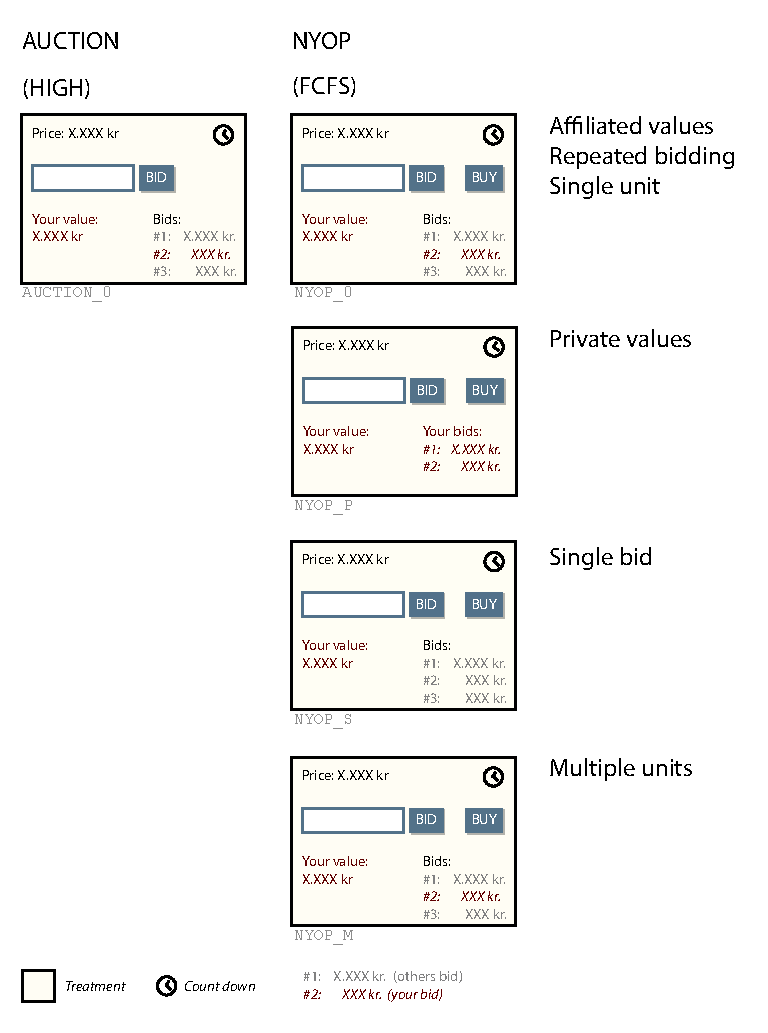
\includegraphics[width=0.85\textwidth]{Figures/Treatments}
			\label{fig:treatments}
	\end{figure}
	
	\newpage
	
	\subsection{Order of treatments}
	\label{app:order_treatments}
	
	\begin{table}[ht]
		\caption{Ordering of treatments (randomised)}
		\begin{tabular}{l | l | l | l | l}
			%{\bf a} 	& {\bf b} 		& {\bf c} 		& {\bf d} 		& {\bf e} \\
			$AUCTION_0$	& $AUCTION_0$ 	& $AUCTION_0$ 	& $NYOP_M$ 		& $NYOP_S$ 	\\
			$NYOP_0$ 	& $NYOP_M$		& $NYOP_P$		& $NYOP_P$		& $NYOP_M$	\\
			$NYOP_P$ 	& $NYOP_S$		& $NYOP_M$		& $NYOP_0$		& $NYOP_0$	\\
			$NYOP_S$	& $NYOP_P$		& $NYOP_0$		& $NYOP_S$		& $NYOP_P$	\\
			$NYOP_M$	& $NYOP_0$		& $NYOP_S$		& $AUCTION_0$	& $AUCTION_0$	
		\end{tabular}
		\label{tab:order}
	\end{table}
	
	\subsection{Example of payments}
	\label{app:example_payment}

	\begin{table}[ht]
		\caption{Examples illustrating a buyer's payment at the end of each round}
		\begin{tabular}{p{0.47\textwidth}  p{0.47\textwidth}}
			{\bf Example 1} (NYOP): 	& {\bf Example 2} (NYOP):  		\\
			Value of buyer: 200 		& Value of buyer: 400 			\\
			Threshold level: 300 		& Threshold level: 300 			\\
			Posted price: 450 			& Posted price: 500 			\\
			The buyer does not manage to purchase the item. His/her payment is 0 kr. & The buyer is first and bids 350 thereby purchasing the item. His/her payment is $\frac{400-350}{10}=5$ kr. \\
			\multicolumn{2}{c}{} \\
			{\bf Example 3} (NYOP):  	& {\bf Example 4} (Auction): 	\\
			Value of buyer: 600 		& Value of buyer: 600  			\\
			Threshold level: 300  		& Posted price: 500  			\\
			Posted price: 500  			&  								\\
			The buyer is first and purchases the item at the posted price. His/her payment is $\frac{600-500}{10}=10$ kr. & The buyer bids 550 and the highest competing bid is 450. The buyer wins the item. His/her payment is $\frac{600-450}{10}=15$ kr. \\
		\end{tabular}
		\label{tab:payment}
	\end{table}

	\subsection{Expected payments}
	\label{app:expected_payment}
	
	Assuming that buyers bid their true value, then in one round of the $AUCTION_0$ treatment the expected payment is the following. Where payment is the difference in expected values between the highest and second highest value distributed on $U[0,1]$ and then readjusted to fit the distribution described in section~\ref{sec:design}:
	\[ \mathbb{E}[\mbox{payment if highest bidder}] \times \mbox{Prob}[\mbox{highest bidder}] \] 
	\[  = \left( \mathbb{E}[a_t] + (\mathbb{E}[Y^{(1)}]-\mathbb{E}[Y^{(2)}]) 400 \right) \times \mbox{Prob}[x_i \ge Y^{(1)}] \] 
	\[	= \left( 800 + \left(\frac{N}{N+1} - \frac{N-1}{N+1}\right)400 \right) \times \frac{1}{N} = 173 \approx 17\mbox{ kr.} \]
	
	Assuming 1) truthful bidding, 2) that buyers are rational (e.g. never bid above the posted price) and 3) the fasted buyer is random (e.g. every buyer equally likely to be the fastest). Then in one round of the $NYOP_0$, the $NYOP_P$ or the $NYOP_S$ treatment the expected payment is:
	\[ \mathbb{E}[\mbox{payment if fastest bidder}] \times \mbox{Prob}[\mbox{fastest bidder}] \] 
	\[  = \left( \mbox{Prob}[\mbox{Value} \ge \mbox{Exp. threshold level}] \times \mathbb{E}[\max\{\mbox{Exp. value}, \mbox{Posted price}\}] \right) \times \frac{1}{N} \] 
	\[  = \left( \mbox{Prob}[x_i \ge \mathbb{E}[\tau]] \times \mathbb{E}[\max\{\mathbb{E}[x_i], p\}]  \right) \times \frac{1}{N} \] 
	\[  = \left( \mbox{Prob}[x_i \ge \mathbb{E}[\tau]] \times ( \mbox{Prob}[\mathbb{E}[x_i] < p] \mathbb{E}[x_i] + \mbox{Prob}[\mathbb{E}[x_i] \ge p] p ) \right) \times \frac{1}{N} \] 
	\[  = \left( \left(1-\frac{N-1}{(N+1)2}\right) \times \left( \frac{N-1}{N} \mathbb{E}[x_i] + \frac{1}{N} p \right) \right) \times \frac{1}{N} \] 
	\[  = \left( \left(1-\frac{N-1}{(N+1)2}\right) \times \left( \frac{N-1}{N} (800+400/2) + \frac{1}{N} \left(800+\frac{N-1}{N+1}400\right) \right) \right) \times \frac{1}{N} \] 
	\[	= 135 \approx 14\mbox{ kr.} \]
	
	In a $NYOP_M$ treatment with same assumption as above, but with $ceil(N/2)=3$ items for sale, then the expected payment in one round is:
	\[ \mathbb{E}[\mbox{payment if fastest bidders}] \times \mbox{Prob}[\mbox{fastest bidders}] \] 
	\[  = \left( \left(1-\frac{N-1}{N+1}\frac{1}{2}\right) \times \left( \frac{N-1}{N} (800+400/2) + \frac{1}{N} \left(800+\frac{N-1}{N+1}400\right) \right) \right) \times \frac{ceil(N/2)}{N} \] 
	\[	= 405 \approx 41\mbox{ kr.} \]


\end{document}

